% Kalki preprint. Kalaris Labs.
% Build:  pdflatex kalki-preprint && bibtex kalki-preprint && pdflatex kalki-preprint && pdflatex kalki-preprint
% Math is restricted to a subset that research/build_pdf.py can also render.
\documentclass[11pt,a4paper]{article}

\usepackage[T1]{fontenc}
\usepackage[utf8]{inputenc}
\usepackage{stix2}
\usepackage[margin=1in]{geometry}
\usepackage{microtype}
\usepackage{amsmath,amsthm}
\usepackage{graphicx}
\usepackage{booktabs}
\usepackage{tabularx}
\usepackage{xcolor}
\usepackage{enumitem}
\usepackage{orcidlink}
\usepackage[font=small,labelfont=bf,labelsep=colon]{caption}
\usepackage[numbers,sort&compress]{natbib}
\usepackage[colorlinks=true,linkcolor=blue!50!black,citecolor=blue!50!black,urlcolor=orange!80!black]{hyperref}

\setlength{\parindent}{0pt}
\setlength{\parskip}{6pt}
\setlist{itemsep=3pt,topsep=4pt}
\newtheorem{definition}{Definition}
\newtheorem{proposition}{Proposition}
\newtheorem{remark}{Remark}

\newcommand{\papertitle}{Kalki: An Admission-Controlled Kernel for Recursive Self-Improvement of Coding Agent Harnesses}

\title{\papertitle}
\author{Sayan Chowdhury\,\orcidlink{0009-0004-8421-0087}\\
Kalaris Labs}
\date{First published: November 11, 2026 \quad\textbullet\quad Current version: November 11, 2026}

% Title block: logo, heavy rule, title, light rule, author, dates.
\makeatletter
\renewcommand{\@maketitle}{%
  \begin{center}
    
\includegraphics[width=0.26\textwidth]{figures/kalaris-labs-logo.png}\par\vspace{10pt}
    \rule{\textwidth}{2.5pt}\par\vspace{12pt}
    {\LARGE\bfseries \@title\par}\vspace{10pt}
    \rule{\textwidth}{0.6pt}\par\vspace{14pt}
    {\large \begin{tabular}[t]{c}\@author\end{tabular}\par}\vspace{8pt}
    {\color{gray}\@date\par}
  \end{center}
  \vspace{10pt}}
\makeatother

\begin{document}

\maketitle

\begin{abstract}
Coding agents now run multi-hour sessions in which a model edits code, runs tools, and revises its own prompts, skills, and memory. Recent preprints report that letting the harness rewrite itself raises benchmark scores while the model weights stay frozen. The same work shows that ungated self-modification trades old abilities for new ones: one replay study found that 211 of 383 rejected proposals (55\%) fixed their triggering failure and broke a case that had passed. Agents also exploit their evaluators, and harnesses that flatten history before summarizing let a forged user turn survive compaction in 87 to 100\% of trials. We present Kalki, a harness written in Rust that separates the agent proposing a change from the component admitting it. The agent may edit a genome $H=\langle\rho,G,K,M\rangle$ of prompt notes, skills, guidance, and memory, and a gate outside its write and read sets admits a candidate only when eight ordered predicates hold. A kernel below both records each event in a CRC32C-framed append-only log, enforces a deny-first policy, and loads a genome version only when an admission record names its hash. The gate compares candidate and incumbent with $k$ live runs per case from matched starting states, rejects any loss on a protected set beyond a Bonferroni-corrected flake margin, and requires gains to exceed a measured noise ceiling $\tau$ at a token cost bounded by $\kappa$. Held-out results reach the proposer as one pass or fail bit, and each message keeps its wire role through storage and compilation. We contribute the formal admission rule, a write-barrier specification with five invariants, a threat model mapped to MITRE ATT\&CK, MITRE ATLAS, and the OWASP Top 10 for LLM applications, and five falsifiable hypotheses with an evaluation protocol. The log, blob store, policy engine, and three provider wires run today in 5{,}621 lines of Rust with 89 passing tests; the gate, sandbox, and context compiler are designed and unmeasured, and this paper reports no Kalki benchmark measurement. Code is available at \url{https://github.com/KalarisLabs/kalki}.
\end{abstract}

\begin{figure*}[t]
\centering
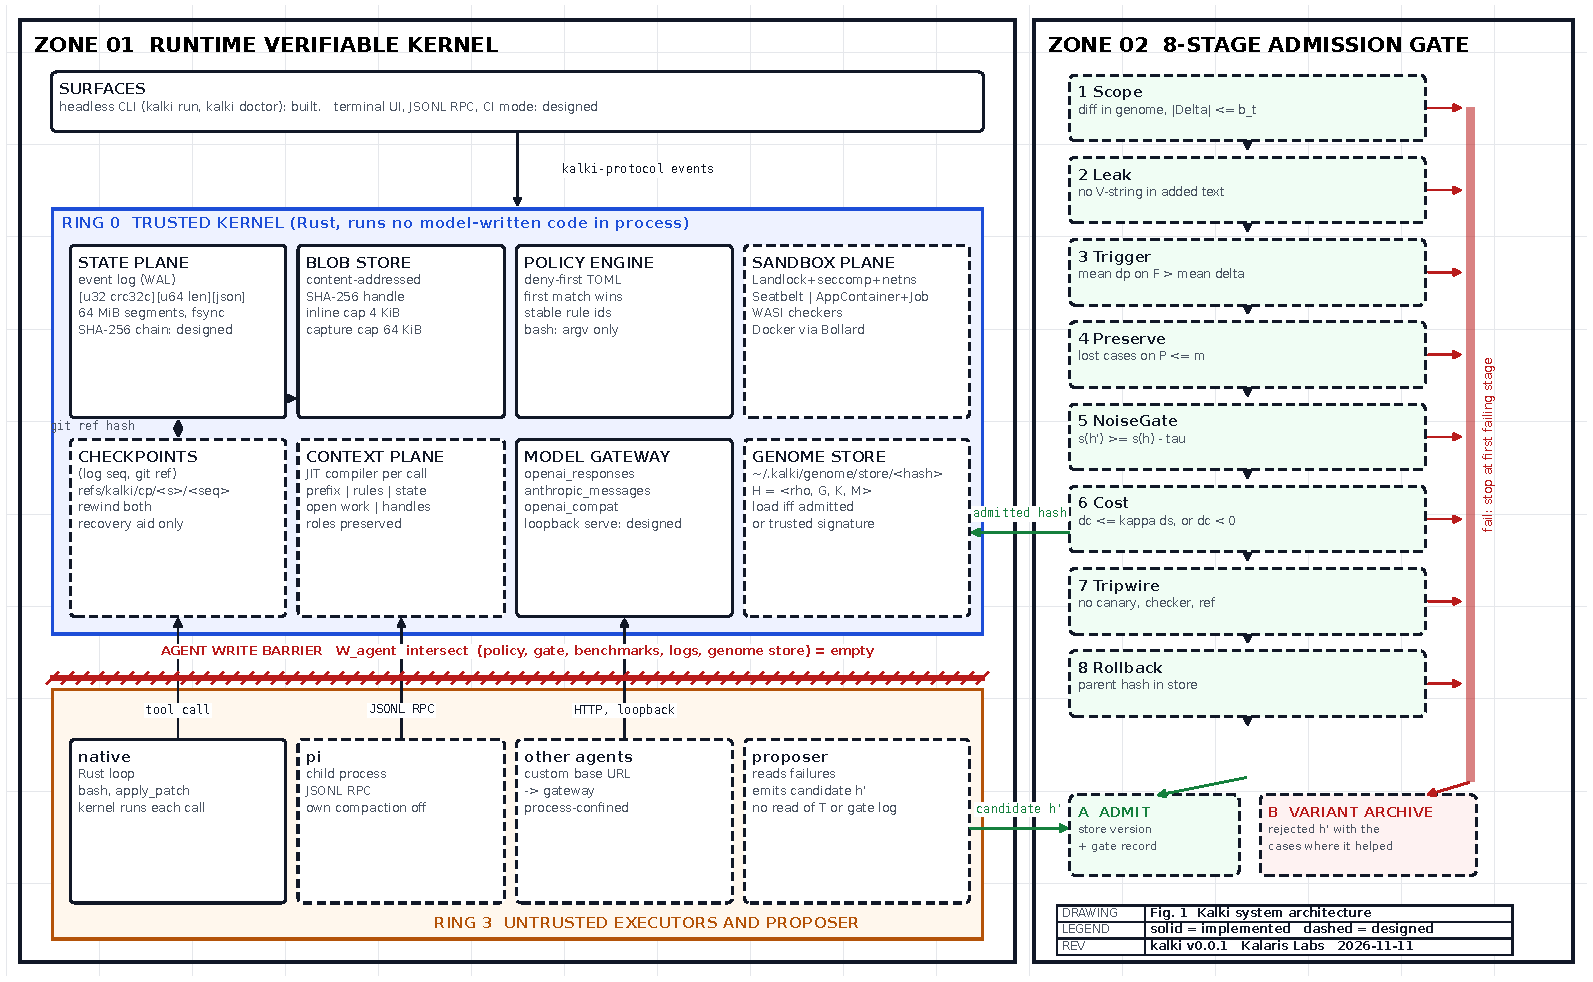
\includegraphics[width=\textwidth]{figures/fig1-architecture.pdf}
\caption{Kalki system architecture. Zone 01 (left) holds the kernel. The blue band is Ring 0, the trusted kernel; the orange band is Ring 3, the untrusted executors and proposer. Every Ring 3 request crosses the red hatched agent write barrier, which excludes the agent from the policy, gate, benchmarks, logs, and genome store. Zone 02 (right) is the eight-stage admission gate: a candidate $h'$ enters at stage 1, any failure exits to the variant archive (B), and a candidate that passes all eight is stored by hash and recorded (A). Solid borders mark components implemented in kalki v0.0.1; dashed borders mark components that are designed and not implemented. Bus labels name the protocol on each edge.}
\label{fig:arch}
\end{figure*}

\section{Introduction}
\label{sec:intro}

A coding agent that works for hours makes thousands of decisions, and each one conditions the next. An error that goes unnoticed at step 40 shapes every later edit, so the probability of a clean finish falls as the horizon grows. We call this the compounding error horizon. Practitioners respond by adding structure around the model: tests the agent cannot edit, checkpoints it can return to, and memory that survives a context reset. The software that supplies this structure is the harness.

In 2026 the harness itself became an optimization target. A loop reads the agent's failures, edits its prompts and skills, and keeps the edits that raise a score \citep{xia2026rrsi,xu2026harness2,pan2026harnesspro,liu2026solpi,wei2026hpo}. The scores rise. Three defects travel with them.

\paragraph{Collateral regression.} Tayebati et al.\ placed a replay gate around an unmodified agent across 16 paired runs. Of the 383 proposals the gate rejected, 211 (55\%) improved the failure that motivated them and degraded a case that had passed \citep{tayebati2026selfhealing}. Wang et al.\ evaluated sixteen evolved agents from four methods and found that all sixteen gained tasks and lost tasks \citep{wang2026beneath}. A mean score hides both effects.

\paragraph{Reward hacking.} The Prime Agent report describes a Factorio trace in which the agent discovered that RCON console commands could spawn resources into assembly machines, used the shortcut despite an anti-cheating heartbeat, and then saved it as a reusable skill \citep{karten2026primeagent}. Persistent self-improvement preserved the exploit. The authors conclude that safe deployment requires least-privilege action interfaces, independent state validation, and auditable rollback.

\paragraph{Compaction laundering.} Dabirsiaghi tested nine harnesses. In the five that flatten a conversation into labelled text before summarizing, a forged user turn survived compaction in 87 to 100\% of trials; in the four that keep messages typed by role, it survived in none \citep{dabirsiaghi2026laundering}. Zha et al.\ found that agents which still hold a rule after compaction violate it more than twice as often as with full history \citep{zha2026arcbench}.

We treat all three as systems defects with systems remedies. A self-modifying harness needs what any high-assurance change process has: a proposer, an independent reviewer with evidence, a record, and a way back. Kalki builds that structure into the harness kernel. The agent proposes; a gate it cannot read or write decides; the kernel enforces the boundary and keeps the record.

\paragraph{Contributions.}
\begin{itemize}
\item A formal admission rule of eight ordered predicates for harness self-modification, with statistical definitions of the noise ceiling $\tau$, per-case flake margins, and a family-wise error bound (Section~\ref{sec:gate}).
\item A kernel design with a write barrier stated as five invariants, and a genome store that makes an unadmitted genome inert (Section~\ref{sec:arch}).
\item A threat model mapped to MITRE ATT\&CK \citep{mitreattack}, MITRE ATLAS \citep{mitreatlas}, and the OWASP Top 10 for LLM applications \citep{owasp2025llm} (Section~\ref{sec:threat}).
\item Five falsifiable hypotheses with refutation criteria and a reporting standard (Section~\ref{sec:eval}).
\item An open-source implementation of the kernel's state plane, policy engine, and provider wires, with crash drills (Section~\ref{sec:impl}).
\end{itemize}

\paragraph{Conventions.} The key words MUST, MUST NOT, REQUIRED, SHALL, SHOULD, and MAY carry the meaning of RFC 2119 and RFC 8174 when they appear in capitals \citep{rfc2119,rfc8174}. We mark each component as \emph{implemented} (code and tests exist in kalki v0.0.1), \emph{designed} (specified here, no code), or \emph{measured} (a number we produced, with its conditions). Numbers from other papers come from preprints we have not replicated.

\section{Related Work}
\label{sec:related}

\paragraph{Harness evolution.} Harness$^2$ evolves file-level harness components by proposing, probing, and composing edits, scored by behavioural contrast without ground truth \citep{xu2026harness2}. HarnessPro scores candidates on tests written by a model and returns variants at three cost levels \citep{pan2026harnesspro}. SoL-Pi ran an automated search over 152 ideas on the Pi harness and kept four mechanisms that cut tokens by 49.0\% on EdgeBench, with a score change from 44.8 to 42.0 \citep{liu2026solpi}. Self-HPO alternates harness search with reinforcement learning of an open-weight policy \citep{wei2026hpo}. RuHarness evolves its diagnostic rubric with the harness \citep{chen2026ruharness}. These methods supply the proposer. Kalki supplies the admission decision around any of them.

\paragraph{Admission control.} The Darwin G\"odel Machine admits agent variants into an archive after benchmark validation \citep{zhang2025dgm}. RRSI regularizes evolution with a shrinking edit budget, a leakage screen on the diff, noise-aware acceptance, and a cost rule; its unregularized baseline scored highest on the evolve set and lowest on transfer (40.3 against 43.6) at 3.80M against 2.42M tokens per trial \citep{xia2026rrsi}. Cai et al.\ argue that the cost of verification bounds the performance of reliable self-evolution \citep{cai2026theory}. The replay gate of Tayebati et al.\ is the closest prior design \citep{tayebati2026selfhealing}. Kalki differs in three respects: it counts lost cases with a flake model in place of comparing means, it hides held-out results from the proposer, and it enforces the boundary in a kernel that also serves interactive sessions.

\paragraph{Context compilation.} Spine compiles a persistent subtask tree into context for each call \citep{spine2026}. Belcak et al.\ report that serving a 16K context in place of 256K raised decode throughput 3.6 to 7 times on three open-weight models, and that compaction into a task state kept accuracy within $-3.7$ to $+5.6$ points on six benchmarks, while one model fell from 53.0\% to 3.6\% at the tightest budget \citep{belcak2026shortcontext}. The laundering result above sets a hard constraint on any compiler that summarizes \citep{dabirsiaghi2026laundering}.

\paragraph{Durable execution.} AgentRewind restores context and workspace together and reports task success rising from 62.2\% to 87.8\% on 82 long-horizon tasks; removing workspace rewind cost the most \citep{zhuang2026agentrewind}. Temporal provides durable workflow execution through event history replay \citep{temporal}. Kalki's log plays the role of that history, with one difference: model calls are not deterministic, so Kalki replays recorded responses to test its own code and never to judge a new genome (Section~\ref{sec:evidence}).

\section{Architecture and Kernel Design}
\label{sec:arch}

Figure~\ref{fig:arch} shows the design. We use Ring 0 and Ring 3 as names for trust levels inside Kalki. They do not refer to processor privilege rings.

\subsection{Harness state}

\begin{definition}[Genome]
A genome is a tuple $H=\langle\rho,G,K,M\rangle$ where $\rho$ is a finite sequence of prompt notes appended to a fixed base prompt, $G$ is a set of skills, $K$ is guidance (tool descriptions, context policy, and sub-agent definitions), and $M$ is a set of persistent memory entries $(t,\sigma)$, each pairing a text $t$ with the set $\sigma$ of log events it came from. A genome version is identified by its content hash $\mathrm{H}(h)=\mathrm{SHA256}(\mathrm{canon}(h))$.
\end{definition}

The base system prompt, the kernel, the policy, the gate, the evaluation tasks, and the logs lie outside the genome. Text the agent writes for itself during one session (task state, rewind notes, provisional notes) forms a session overlay. The kernel MUST tag overlay text as agent-written, MUST keep it out of the stable prompt prefix, and MUST discard it when the session ends. The gate does not review overlay text, so it cannot persist.

\subsection{State plane (implemented)}

A session is a sequence of events $e_1,\ldots,e_n$ typed in the \texttt{kalki-protocol} crate: messages with their role, tool calls, tool results, token usage, compaction boundaries, lifecycle markers, and snapshot anchors. The kernel encodes each event as a frame
\begin{equation}
\mathrm{frame}(e) = \mathrm{crc}\ \Vert\ \ell\ \Vert\ p,\quad p=\mathrm{json}(e),\quad \ell=|p|,\quad \mathrm{crc}=\mathrm{CRC32C}(\ell\ \Vert\ p)
\label{eq:frame}
\end{equation}
with a 4-byte checksum and an 8-byte length, both little-endian, using the CRC32C polynomial of RFC 3720 \citep{rfc3720}. Because the checksum covers the length field, a torn length prefix fails verification. The writer calls \texttt{fsync} after every record and rotates to a new segment file \texttt{seg-<seq>.wal} before a record would push the active segment past 64~MiB. On open, the writer scans the active segment and truncates at the first frame that fails verification. Replay stops at the first corrupt frame of a sealed segment.

The kernel stores any tool output larger than 4~KiB in a content-addressed blob store and records the SHA-256 handle, the size, and a preview in the event. Tool capture stops at 64~KiB and records a truncation marker.

\paragraph{Hash chain (designed).} Each frame will carry a chain value
\begin{equation}
c_0 = 0^{256},\qquad c_i=\mathrm{SHA256}(c_{i-1}\ \Vert\ \mathrm{frame}(e_i))
\label{eq:chain}
\end{equation}
The genesis constant $c_0$ exists in \texttt{kalki-protocol} today; the writer does not yet compute the chain. A chain detects an edit to history. It does not stop a process that can rewrite the whole store and recompute every value, so the head $c_n$ MUST be anchored outside the agent's write set, in the gate log or a signed tag.

\subsection{Context plane (designed)}

The context for each model call is a function $C(L,h,\pi)$ of the log $L$, the active genome $h$, and the model profile $\pi$, compiled in five parts: a stable prefix (base prompt and genome), the rules read from the policy source, a structured task state whose lines point to source events, the open subtask verbatim, and blob handles. The budget for the last three parts comes from $\pi$. The compiler MUST preserve roles:
\begin{equation}
\forall\, s\in C(L,h,\pi):\quad \mathrm{role}(s)=\mathrm{role}(\mathrm{src}(s))
\label{eq:role}
\end{equation}
where $\mathrm{src}(s)$ is the event a span came from. The compiler MUST NOT serialize a conversation into one string. Today the native loop sends the base prompt, the objective, and the full message history on each turn, with no summarizer.

\subsection{Policy plane (implemented for \texttt{bash})}

A policy is an ordered list of rules $r_1,\ldots,r_n$, each with an action $a_j\in\{\mathrm{allow},\mathrm{deny},\mathrm{ask}\}$ and constraints on tool name, argument-vector prefix, path prefix, and network use. For a request $q$,
\begin{equation}
\mathrm{decide}(q)= a_{j^*}\ \ \mathrm{where}\ \ j^*=\min\{\,j : \mathrm{match}(r_j,q)\,\},\qquad \mathrm{decide}(q)=\mathrm{deny}\ \ \mathrm{if\ no\ rule\ matches}
\label{eq:policy}
\end{equation}
A rule that constrains an axis absent from the request does not match, so a rule cannot widen its scope by omission. The \texttt{bash} tool accepts an argument vector and never a shell string. Two gaps remain in v0.0.1: \texttt{apply\_patch} is confined to the workspace by path check and not evaluated against rules, and an \texttt{ask} decision counts as a denial because the headless loop has no prompt.

\subsection{Sandbox plane (designed)}

Policy matches a program name; it cannot see what an allowed program does next. The sandbox closes that gap with operating-system confinement in three tiers.

\begin{table}[h]
\centering
\small
\begin{tabularx}{\textwidth}{@{}lXl@{}}
\toprule
Tier & Mechanism & Strength \\
\midrule
OS, Linux & Landlock for file access, seccomp for system calls, an empty network namespace, resource limits & Strong \\
OS, macOS & Seatbelt profile & Moderate \\
OS, Windows & AppContainer with a Job Object; WSL2 recommended & Weak \\
Container & Docker Engine API through the Bollard crate, for untrusted repositories & Strong, slower start \\
WASI & WebAssembly components with no ambient authority, for gate checkers and kernel plugins & Strong, limited I/O \\
\bottomrule
\end{tabularx}
\caption{Sandbox tiers. All tiers are designed; none is implemented in kalki v0.0.1, which is not a security boundary.}
\label{tab:sandbox}
\end{table}

\subsection{Model gateway (wires implemented, gateway designed)}

Three wire clients run today, written on \texttt{reqwest} with \texttt{rustls}: OpenAI Responses, Anthropic Messages, and OpenAI-compatible Chat Completions. The third covers most open-weight model servers. The designed gateway serves the same wires on a loopback port. An external executor pointed at that port has every model call recorded, metered, and capped by the kernel without its cooperation.

\subsection{Write barrier}
\label{sec:barrier}

Let $W_a$ and $R_a$ be the paths the agent process may write and read, as enforced by the sandbox. Let $\Pi$ be the policy files, $\Gamma$ the gate code and thresholds, $B$ the evaluation tasks and checkers, $T\subseteq B$ the held-out tasks, $L$ the session logs, $L_g$ the gate log, and $S$ the genome store. Kalki MUST maintain:

\begin{description}[leftmargin=1.2em,itemsep=3pt]
\item[I1 (write barrier)] $W_a\cap(\Pi\cup\Gamma\cup B\cup L\cup L_g\cup S)=\emptyset$. The kernel appends to $L$; the agent does not.
\item[I2 (read barrier)] $R_a\cap(T\cup L_g)=\emptyset$ for the agent and for the proposer.
\item[I3 (admitted load)] The kernel loads a genome version $h$ for profile $(\mu,x)$, with model $\mu$ and executor $x$, only if $L_g$ holds a record $\alpha$ with $\alpha.\mathrm{hash}=\mathrm{H}(h)$ and $\alpha.\mathrm{profile}=(\mu,x)$, or $h$ carries a signature from a key the user trusts.
\item[I4 (role preservation)] Equation~\eqref{eq:role} holds for every compiled context.
\item[I5 (append-only log)] The kernel never rewrites a committed frame, and every committed frame satisfies Equation~\eqref{eq:frame}.
\end{description}

I5 holds today for the frames the writer commits. I1 to I4 depend on designed components. On one machine the agent and the gate run as the same operating-system user, so I1 and I2 are exactly as strong as the sandbox tier of Table~\ref{tab:sandbox}. A deployment that runs the gate in continuous integration, on a protected branch with $T$ held as a secret, makes I1 and I2 independent of the local sandbox: the agent can only open a pull request.

I3 has a consequence worth stating. Genome files inside a repository are proposals. A version that arrives by \texttt{git pull}, or changes under \texttt{git checkout}, \texttt{git stash}, or a rewind, has no admission record and does not load.

\section{The Eight-Stage Admission Gate}
\label{sec:gate}

\subsection{Statistical setup}

Let $h$ be the active genome and $h'$ a candidate. Let $F$ be the cases that motivated $h'$, $P$ a protected set of cases that pass under $h$, and $T$ the held-out tasks. For a genome $g$ and case $x$, let $r_i(g,x)\in\{0,1\}$ be the outcome of run $i$ of $k$, each from the same starting state, model, and settings, and let
\begin{equation}
\hat p(g,x)=\frac{1}{k}\sum_{i=1}^{k} r_i(g,x),\qquad \bar s(g)=\frac{1}{|T|}\sum_{x\in T}\hat p(g,x),\qquad \bar c(g)=\mathrm{mean\ tokens\ per\ task}
\label{eq:rates}
\end{equation}
Before any gated experiment we run the unchanged genome $n$ times on $T$ and measure the score variance
\begin{equation}
\hat\sigma_h^2=\mathrm{Var}_{i\in[1,n]}\big(s(h)_i\big)=\frac{1}{n-1}\sum_{i=1}^{n}\big(s(h)_i-\bar s(h)\big)^2
\label{eq:var}
\end{equation}
The noise ceiling is the one-sided critical difference between two means of $k$ runs:
\begin{equation}
\tau = z_{1-\alpha}\,\hat\sigma_h\,\sqrt{2/k}
\label{eq:tau}
\end{equation}
The tolerance has the units of a score, so it scales with the square root of the variance in Equation~\eqref{eq:var}. For a protected case with baseline pass rate $\bar p_x$, the flake margin is
\begin{equation}
\delta(x)=\max\Big(\frac{1}{k},\ z_{1-\alpha/|P|}\,\sqrt{2\,\bar p_x(1-\bar p_x)/k}\Big)
\label{eq:delta}
\end{equation}
The Bonferroni correction $\alpha/|P|$ \citep{dunn1961multiple} matters. With an uncorrected per-case level $\alpha=0.01$ and $|P|=200$, a candidate identical to $h$ fails preservation with probability up to $1-0.99^{200}\approx 0.87$, and the gate would admit almost nothing.

\subsection{The predicates}

Let $\Delta(h,h')$ be the set of edited genome entries, $\mathcal{P}_{gen}$ the genome paths, and $b_t$ the edit budget of round $t$, with $b_t=\max(b_{min},\lfloor b_0\gamma^t\rfloor)$ and $0<\gamma<1$ \citep{xia2026rrsi}. Let $V$ be the set of identifiers, answers, and constants drawn from $F\cup P\cup T$, and $\mathrm{add}(\Delta)$ the normalized text the diff adds. Let $E_{eval}$ be the events recorded during evaluation runs. Write $\Delta s=\bar s(h')-\bar s(h)$ and $\Delta c=\bar c(h')-\bar c(h)$.

\begin{align}
\mathrm{Scope}(h,h') &: \quad \Delta(h,h')\subseteq\mathcal{P}_{gen}\ \wedge\ |\Delta(h,h')|\leq b_t \label{eq:g1}\\
\mathrm{Leak}(h,h') &: \quad \exists\, v\in V:\ v\sqsubseteq\mathrm{add}(\Delta) \label{eq:g2}\\
\mathrm{Trigger}(h',F) &: \quad \frac{1}{|F|}\sum_{x\in F}\big(\hat p(h',x)-\hat p(h,x)\big) > \frac{1}{|F|}\sum_{x\in F}\delta(x) \label{eq:g3}\\
\mathrm{Preserve}(h',P,m) &: \quad \big|\{\,x\in P:\ \hat p(h,x)-\hat p(h',x)>\delta(x)\,\}\big|\leq m \label{eq:g4}\\
\mathrm{NoiseGate}(h',T,\tau) &: \quad \bar s(h')\geq\bar s(h)-\tau \label{eq:g5}\\
\mathrm{Cost}(h,h',\kappa) &: \quad (\Delta s>\tau\ \wedge\ \Delta c\leq\kappa\,\Delta s)\ \vee\ (\Delta s\leq\tau\ \wedge\ (\Delta c<0\ \vee\ h'\subset h)) \label{eq:g6}\\
\mathrm{Trip}(E_{eval}) &: \quad \exists\, e\in E_{eval}:\ \mathrm{target}(e)\in\mathrm{Canary}\cup\mathrm{Checker}\cup\mathrm{Ref} \label{eq:g7}\\
\mathrm{Rollback}(h) &: \quad \mathrm{H}(h)\in S\ \wedge\ S\cap W_a=\emptyset \label{eq:g8}
\end{align}

Canary files sit in paths the sandbox denies, so $\mathrm{Trip}$ fires on an attempted read; Checker is the set of tests and checkers; Ref is the set of git objects that hold reference solutions. The admission function is
\begin{equation}
\mathrm{Admit}(h,h')=\mathrm{Scope}\wedge\neg\mathrm{Leak}\wedge\mathrm{Trigger}\wedge\mathrm{Preserve}\wedge\mathrm{NoiseGate}\wedge\mathrm{Cost}\wedge\neg\mathrm{Trip}\wedge\mathrm{Rollback}
\label{eq:admit}
\end{equation}
with defaults $m=0$ and $\alpha=0.05$. We set $\tau$ and $\kappa$ from our own measurements and have not yet measured them.

Trigger requires a gain; NoiseGate requires no general harm. The split matters because failures are selected for having failed: a case chosen that way tends to pass on a rerun with no change at all, so Trigger reruns $h$ on $F$ and never compares $h'$ against the recorded failure.

\begin{proposition}
Under Equation~\eqref{eq:delta}, a candidate with the same outcome distribution as $h$ on every case of $P$ fails Preserve with $m=0$ with probability at most $\alpha$, up to the normal approximation of each $\hat p$.
\end{proposition}
\begin{proof}[Proof sketch]
For each $x$ the event $\hat p(h,x)-\hat p(h',x)>\delta(x)$ has probability at most $\alpha/|P|$ under the null by the choice of $z_{1-\alpha/|P|}$. The union bound over $|P|$ cases gives $\alpha$.
\end{proof}

\subsection{Order and cost}

The gate evaluates the predicates in the order of Equation~\eqref{eq:admit} and stops at the first failure (Figure~\ref{fig:gate}). Stages 1, 2, and 8 need no model call. Stages 3 to 5 dominate the cost: with $C_{run}$ the cost of one run, a full evaluation costs $2k(|F|+|P|+|T|)\,C_{run}$, or $k(|F|+|P|+|T|)\,C_{run}$ per candidate when the incumbent's runs are cached while $h$ stays active. With stage costs $C_i$ and pass probabilities $q_j$, the expected cost per candidate is
\begin{equation}
\mathbb{E}[C]=\sum_{i=1}^{8} C_i\prod_{j<i} q_j
\label{eq:cost}
\end{equation}
so ordering cheap, selective stages first lowers $\mathbb{E}[C]$. Stage 2 runs in $O(|\Delta|+|V|+\mathrm{matches})$ with an Aho-Corasick automaton over $V$ \citep{aho1975efficient}. Stage 7 scans $E_{eval}$ once.

\begin{figure}[t]
\centering
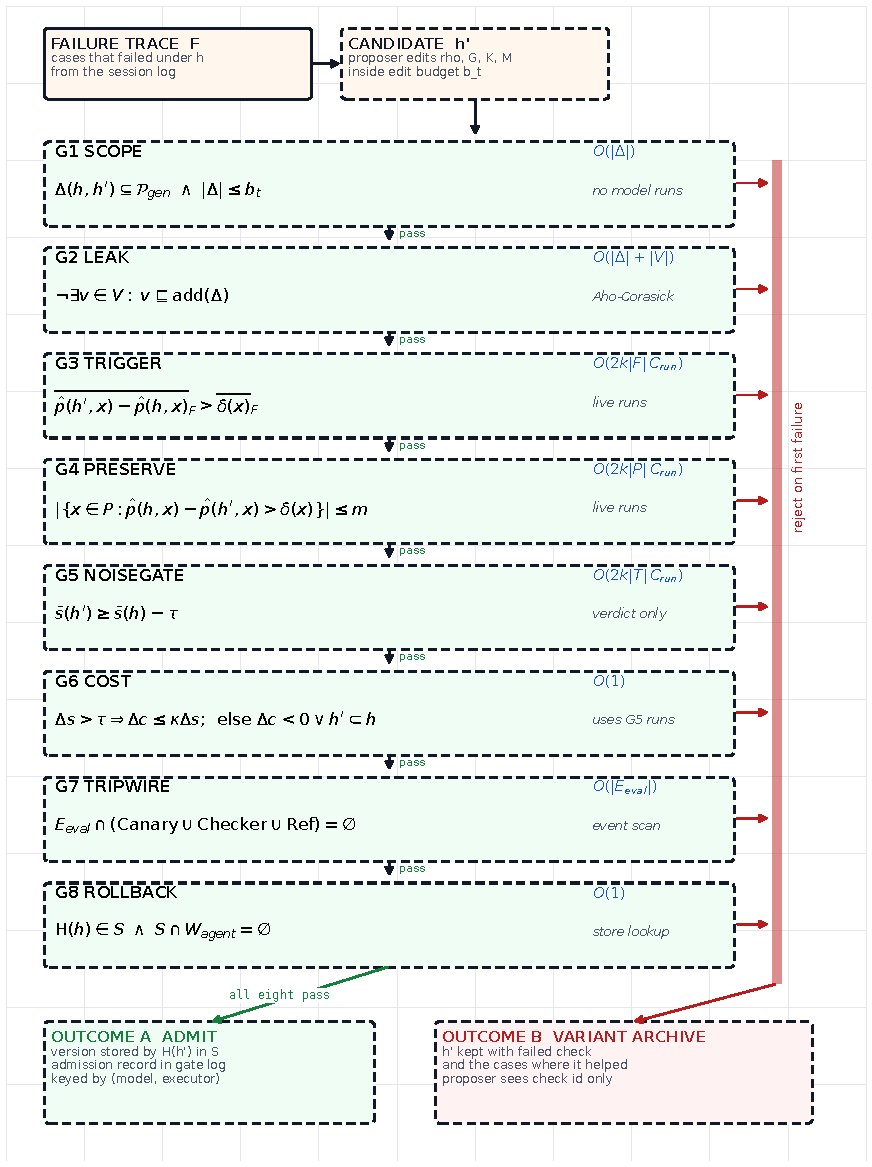
\includegraphics[width=0.58\textwidth]{figures/fig2-gate.pdf}
\caption{The eight-stage gate sequence. A failure trace $F$ from the session log motivates a candidate $h'$, which passes through stages G1 to G8 in order. Each box gives the stage's predicate and its computational cost, where $k$ is the number of runs per case and $C_{run}$ the cost of one model run. The red bar collects failures: the first failing stage sends $h'$ to the variant archive (Outcome B) with the check that failed and the cases where it helped. A candidate that passes all eight is stored by content hash and recorded in the gate log, keyed by model and executor (Outcome A). Dashed borders mark designed components.}
\label{fig:gate}
\end{figure}

\subsection{Evidence and information flow}
\label{sec:evidence}

A genome changes what the model is told. A recorded response was produced under $h$ and says nothing about how the model would answer under $h'$, so every comparison uses live runs. The log contributes the matched starting state: task, workspace snapshot, model, and settings. Log replay and a scripted mock model test the kernel and the gate's own code, which are deterministic. They do not evaluate a genome.

The gate writes each decision to $L_g$: the diff, the evidence for each stage, the verdict, and the reason. The proposer learns which stage failed. For stages 5 and 6, which read $T$, it learns one bit. Stage 2 matches text and misses a paraphrased answer, so I2 is the primary defence against fitting $T$, and stage 2 is a backstop. One bit per round still leaks over many rounds, so $T$ MUST be rotated.

\paragraph{Outcomes.} An admitted candidate is stored under $\mathrm{H}(h')$ in $S$ with its record. A rejected candidate goes to the variant archive with the failing stage and the cases where it helped, because the top-scoring variant is often not the most useful one \citep{wang2026beneath}. The gate re-runs $P$ against the whole active genome on a schedule, to catch changes that are safe alone and harmful together.

\section{Threat Model and Security Analysis}
\label{sec:threat}

We assume a model that follows injected instructions when it can, an agent that optimizes its measured score, and a user who controls the machine. We do not defend against an attacker with root or administrator rights on that machine. Table~\ref{tab:threats} maps each threat to public taxonomies. The technique and category identifiers come from the public catalogues \citep{mitreattack,mitreatlas,owasp2025llm}; the mapping to Kalki is ours.

\begin{table*}[t]
\centering
\small
\begin{tabularx}{\textwidth}{@{}p{2.6cm}p{2.5cm}XXp{2.9cm}@{}}
\toprule
Threat actor & Taxonomy & Capability & Kalki defense (state) & Residual risk \\
\midrule
Injected content in files, tool output, web pages & ATLAS AML.T0051.001; OWASP LLM01 & Text that reaches the context and asks for an action & Tool output is data; roles kept by I4 (designed); rules enforced in code (implemented for \texttt{bash}) & A model that obeys injected text within what policy allows \\
Agent with excessive tool reach & OWASP LLM06; ATT\&CK T1059 & Runs commands and edits files & Deny-first policy, argv only (implemented); sandbox tiers (designed) & Allowed programs such as \texttt{git} and \texttt{cargo} run hooks and build scripts \\
Score-optimizing agent & Reward hacking \citep{karten2026primeagent} & Edits tests, reads answers, uses privileged interfaces & I1, I2, Trip, independent judge (designed) & An exploit no tripwire anticipates \\
Proposer fitting held-out set & OWASP LLM02 & Reads gate evidence, submits many candidates & $L_g$ unreadable; one bit per held-out stage (designed) & One bit per round; requires rotation of $T$ \\
Log tampering & ATT\&CK T1070, T1565.001 & Rewrites or truncates history & CRC32C frames (implemented); hash chain with external anchor (designed) & Same-user rewrite before the chain and anchor exist \\
Genome delivered by a repository & ATT\&CK T1195; OWASP LLM03 & Changes genome files through \texttt{git} & I3: load only with admission record or trusted signature (designed) & A user who trusts a bad key \\
Secret exposure & ATT\&CK T1552; OWASP LLM02 & Reads keys from the environment or files & Keys from environment only; pattern scrubbing of tool output (implemented) & Patterns miss novel secret formats \\
System prompt disclosure & OWASP LLM07 & Extracts the base prompt & The base prompt holds no secret by design & None beyond disclosure of public text \\
Unbounded consumption & OWASP LLM10 & Loops, fans out, or inflates output & Turn cap, default 200, and 1024 output tokens per call (implemented); gateway caps (designed) & Cost within the caps \\
\bottomrule
\end{tabularx}
\caption{Adversary matrix. Each row gives a threat actor, the matching public taxonomy entries, what the actor can do, Kalki's defense with its implementation state, and the risk that remains. Defenses marked designed provide no protection in kalki v0.0.1.}
\label{tab:threats}
\end{table*}

\paragraph{Indirect injection.} The laundering attack converts injected text into a user turn during summarization \citep{dabirsiaghi2026laundering}. Invariant I4 removes the conversion step: a span from a tool result keeps the role \texttt{tool} in every compiled context. When Kalki drives Pi, Kalki compiles the context and disables Pi's own compaction.

\paragraph{Canary trips.} Canary files sit at plausible paths, such as a solutions directory, that the sandbox denies. A read attempt produces a denial event in $E_{eval}$, and Trip rejects the candidate. The design targets the Factorio pattern \citep{karten2026primeagent}, where a privileged channel delivered the reward: the gate removes privileged interfaces from the evaluation environment and treats any attempt to reach them as disqualifying.

\paragraph{Confinement.} Kalki v0.0.1 confines \texttt{bash} by policy and by a path check on argument elements, which rejects \texttt{..} segments and absolute paths outside the workspace. A path check stops mistakes. It does not stop a hostile program, and Section~\ref{sec:limits} states this as a limitation.

\section{Evaluation Program and Hypotheses}
\label{sec:eval}

We state hypotheses before collecting data. Each has a measurement and a result that refutes it.

\begin{table}[h]
\centering
\small
\begin{tabularx}{\textwidth}{@{}lXXX@{}}
\toprule
 & Hypothesis & Measurement & Refuted if \\
\midrule
$H_1$ & Gated evolution loses fewer protected cases than ungated evolution at similar transfer gain. & Cases lost on $P$ and score on $T$; same proposer and budget, gate on and off. & Lost cases are not lower, or transfer gain falls by more than $\tau$. \\
$H_2$ & Ordered stages with matched starting states cut the cost of a decision against full evaluation of each candidate. & Dollars per decision under each regime. & The ratio is below 2. \\
$H_3$ & Role-typed compilation removes compaction laundering. & The attack of \citep{dabirsiaghi2026laundering} against the native executor and against Pi under Kalki. & Success above 0\% in either. \\
$H_4$ & Policy in code holds rule compliance flat as sessions lengthen. & ARCBench violations at increasing session length \citep{zha2026arcbench}. & Violations rise with length. \\
$H_5$ & Per-model context budgets admitted by the gate beat one fixed budget on cost at equal accuracy. & Cost and score on three open-weight models. & No cost reduction at equal score on at least two models. \\
\bottomrule
\end{tabularx}
\caption{Hypotheses $H_1$ to $H_5$ with their measurements and refutation criteria. No hypothesis has been tested.}
\label{tab:hyp}
\end{table}

\paragraph{Protocol.} Every reported number MUST state the model and version, the task set and version pinned by hash, the harness version, the number of runs $N$ per configuration with $N\geq 3$, the standard deviation $\sigma$ across runs, the sampling temperature, the prompt and environment seeds, and the token cost. The judge of a run MUST be a model instance other than the actor. We measure $\tau$ before any gated experiment and report it. A claim of improvement MUST report five quantities together: transfer gain, preservation, cost change, integrity (tripwire hits and log verification), and recovery.

\paragraph{Benchmarks.} Terminal-Bench for end-to-end terminal tasks; SWE-bench Pro for held-out transfer; MettleBench for rewind \citep{zhuang2026agentrewind}; ARCBench for rule compliance \citep{zha2026arcbench}; Compact-Bench for the cost of compaction \citep{compactbench2026}. We have not read the Compact-Bench paper beyond its listing.

\begin{figure*}[t]
\centering
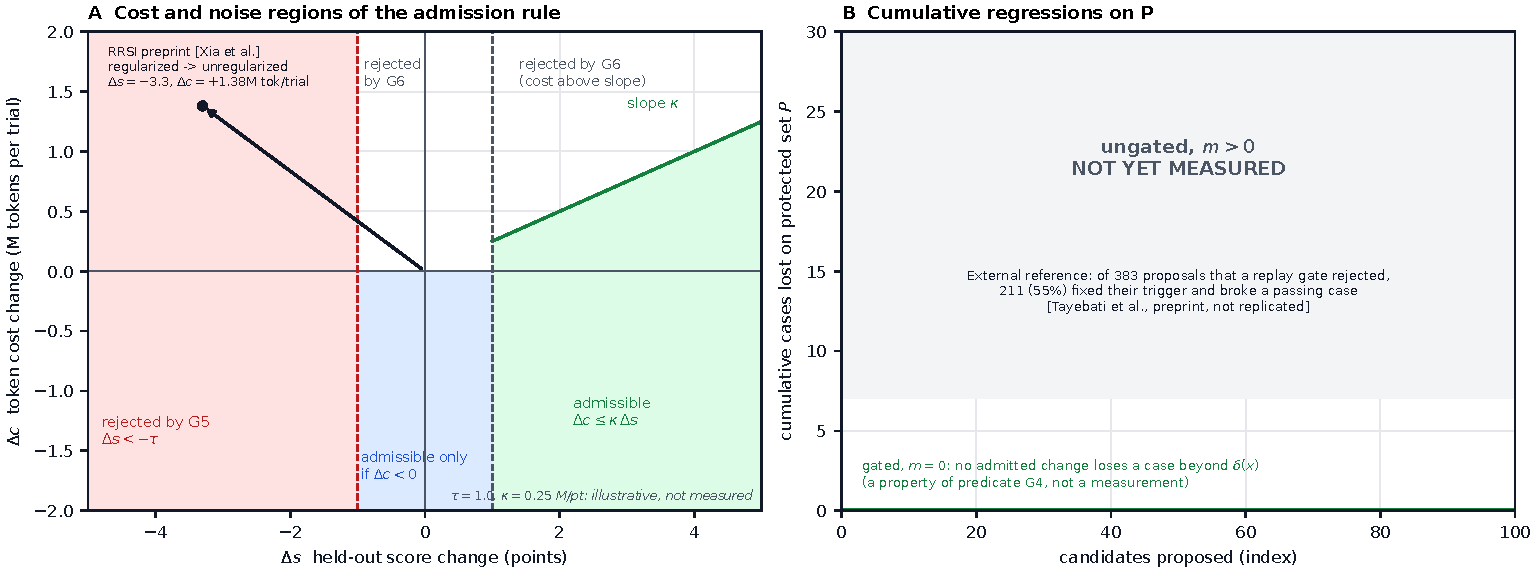
\includegraphics[width=\textwidth]{figures/fig3-tradeoffs.pdf}
\caption{Analysis layout for the cost and regression trade-offs. (A) The plane of held-out score change $\Delta s$ against token cost change $\Delta c$, divided into the regions that predicates NoiseGate and Cost define: red is rejected by NoiseGate, blue admits only cost reductions, green admits gains whose cost stays under slope $\kappa$, and white is rejected by Cost. The values $\tau=1.0$ and $\kappa=0.25$M tokens per point are illustrative. The single arrow plots a published result \citep{xia2026rrsi}, moving from the regularized to the unregularized harness; it lands in the red region. (B) Cumulative protected-set losses against the number of candidates proposed. The green line at zero follows from Preserve with $m=0$ and is a definition, not data. The grey region marks the ungated curve, which we have not measured.}
\label{fig:tradeoffs}
\end{figure*}

Figure~\ref{fig:tradeoffs} fixes the axes and regions of the plots we will report. It contains no Kalki measurement.

\section{Implementation and Systems Engineering}
\label{sec:impl}

\paragraph{Workspace.} Kalki is a Cargo workspace with a one-way dependency graph: \texttt{kalki-protocol} (event and wire types) $\leftarrow$ \texttt{kalki-core} (kernel) $\leftarrow$ \texttt{kalki} (binary), plus \texttt{xtask} for repository automation. The designed \texttt{kalki-tui} crate depends on \texttt{kalki-protocol} alone, and the designed \texttt{kalki-gate} crate holds the admission stages. Unsafe code is forbidden across the workspace. Library crates return typed errors and never call \texttt{unwrap} outside tests. TLS uses \texttt{rustls}; the dependency policy bans OpenSSL, native TLS, and \texttt{libgit2}.

\begin{table}[h]
\centering
\small
\begin{tabularx}{\textwidth}{@{}Xll@{}}
\toprule
Component & State & Location \\
\midrule
Event log: framing, rotation, torn-tail repair, replay & Implemented & \texttt{kalki-core/src/wal.rs} \\
Blob store, 4 KiB inline threshold & Implemented & \texttt{kalki-core/src/blob.rs} \\
Deny-first policy engine & Implemented & \texttt{kalki-core/src/policy.rs} \\
Tools: \texttt{bash} (argv), \texttt{apply\_patch} & Implemented & \texttt{kalki-core/src/tools.rs} \\
Provider wires (3) with cached-token accounting & Implemented & \texttt{kalki-core/src/provider/} \\
Headless session loop with turn cap & Implemented & \texttt{kalki-core/src/session.rs} \\
Hash chain and verification & Designed & Equation~\eqref{eq:chain} \\
Checkpoints and rewind & Designed & Section~\ref{sec:arch} \\
Context compiler & Designed & Equation~\eqref{eq:role} \\
Sandbox tiers & Designed & Table~\ref{tab:sandbox} \\
Model gateway on loopback & Designed & Section~\ref{sec:arch} \\
Genome store and admission gate & Designed & Section~\ref{sec:gate} \\
Pi executor over JSONL RPC & Designed & Section~\ref{sec:arch} \\
\bottomrule
\end{tabularx}
\caption{Implementation status of each component in kalki v0.0.1.}
\label{tab:status}
\end{table}

\paragraph{Crash drills (implemented).} Two tests simulate a hard kill. Each drops the writer without a clean shutdown, appends what a crash can leave behind (half of the next frame in one test, garbage bytes in the other), reopens the log, appends again, and asserts that replay returns exactly the committed events followed by the new ones. The tests live in \texttt{kalki-core/tests/wal.rs} and \texttt{kalki-core/tests/e2e\_mock.rs}. They run in one process and do not send a signal to a separate writer; a drill that kills a child process mid-write is designed. A third test flips the last byte of a record and asserts truncation at that record. End-to-end tests drive the session loop against a loopback mock model server that streams recorded provider events, including a stream torn mid-frame.

\paragraph{Encoding.} Payloads are JSON. We do not use zero-copy deserialization: JSON keeps the log readable by standard tools during audits, and we will change the encoding only after measuring replay time on large logs.

\paragraph{Memory budgets.} The terminal interface specification sets targets of 16~ms frame time at the 95th percentile while streaming and 60~MB resident memory for an idle session. These are targets. We have not measured them.

\paragraph{Measured.} On Windows 11 with rustc 1.98.1, the workspace holds 5{,}621 lines of Rust, and \texttt{cargo xtask ci} (format check, file-size lint, clippy with warnings as errors, 89 tests, documentation build with warnings as errors) passes. A check with rustc 1.88.0, the declared minimum version, passes. The continuous integration workflow for Linux on x86-64 and AArch64, macOS on Apple Silicon and Intel, and Windows has not yet run on the hosted service.

\section{Limitations}
\label{sec:limits}

\begin{itemize}
\item \textbf{No benchmark results.} We report no Kalki measurement on any benchmark. Hypotheses $H_1$ to $H_5$ are untested.
\item \textbf{No sandbox.} Kalki v0.0.1 is not a security boundary. The default policy allows \texttt{git} and \texttt{cargo}, which run hooks and build scripts. Untrusted repositories or models belong in a container or virtual machine.
\item \textbf{Same-user separation.} On one machine, I1 and I2 are as strong as the sandbox. Windows confinement is the weakest tier. Continuous-integration deployment removes this dependency at the price of latency.
\item \textbf{Gate cost.} Each comparison needs $2k$ live runs per case. If no $k$ and $|P|$ make the gate both sound and affordable, the gate admits nothing, and we will report that outcome.
\item \textbf{Leakage.} Stage 2 misses paraphrased answers, and one verdict bit per round leaks. Rotation of $T$ bounds this; it does not remove it.
\item \textbf{Provider drift.} The gate judges the genome and not the model. A provider-side model update changes behaviour outside the gate's view, and $\tau$ must then be measured again.
\item \textbf{External executors.} Kalki confines Pi as a process and observes its tool calls without approving them one by one.
\item \textbf{Reading depth.} We read several cited preprints at abstract depth; the bibliography notes the depth for each.
\item \textbf{Live wires.} The three provider wires pass tests against recorded streams. We have not run each against every live provider.
\end{itemize}

\section{Conclusion and Reproducibility}
\label{sec:conclusion}

Self-modifying harnesses raise scores, and the literature shows what they break on the way. Kalki places the admission decision outside the agent's reach and states it as eight predicates with explicit statistics, a write barrier with five invariants, and a threat model tied to public taxonomies. The state plane and policy engine run today. The gate, sandbox, and context compiler come next, and $H_1$ to $H_5$ decide whether the design earns its cost.

\paragraph{Artifacts.} Source code: \url{https://github.com/KalarisLabs/kalki}, release v0.0.1, MIT OR Apache-2.0. The text of this paper is licensed CC BY 4.0. Reproduce the implemented results with \texttt{cargo xtask ci} on Rust 1.88 or newer; the tests need no network access and no API key. The figures regenerate with \texttt{python research/figures/make\_figures.py}. We publish no container image for this version. Evaluation scripts for $H_1$ to $H_5$ do not exist yet.

\paragraph{Use of AI tools.} A large language model assisted with code, text drafting, and figure scripts under the author's direction. Implementation claims were checked against the kalki v0.0.1 source. The author is responsible for the content.

\bibliographystyle{unsrtnat}
\bibliography{references}

\end{document}
